\subsection{Dependency graphs and topological sorting}

Topological sorting is an operation many programmers well familiar with: this is what ``make'' tool
do when it find an order of items to process.
Items not dependent of anything can be processed first.
The most dependent items at the end.

Dependency graph is a graph and topological sorting is such a ``contortion'' of the a graph,
when you can see an order of items.

For example, let's create a sample graph in Wolfram Mathematica:

\begin{lstlisting}
In[]:= g = Graph[{7 -> 1, 7 -> 0, 5 -> 1, 3 -> 0, 3 -> 4, 1 -> 2, 1 -> 6, 
   1 -> 4, 0 -> 6}, VertexLabels -> "Name"]
\end{lstlisting}

\begin{figure}[H]
\centering
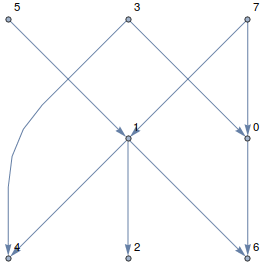
\includegraphics[scale=0.6]{SMT/tsort/math.png}
\caption{}
\end{figure}

Each arrow shows that an item is needed by an item arrow pointing to, i.e., if ``a -> b'', then item ``a'' must be first
processed, because ``b'' needs it, or ``b'' depends on ``a''.

How Mathematica would ``sort'' the dependency graph?

\begin{lstlisting}
In[]:= TopologicalSort[g]
Out[]= {7, 3, 0, 5, 1, 4, 6, 2}
\end{lstlisting}

So you're going to process item 7, then 3, 0, and 2 at the very end.

\href{https://en.wikipedia.org/wiki/Topological_sorting}{The algorithm in the Wikipedia article}
is probably used in the ``make'' and whatever IDE you use for building your code.

Also, many UNIX platforms had separate ``tsort'' utility:
\url{https://en.wikipedia.org/wiki/Tsort}.

How would ``tsort'' sort the graph? I'm making the text file with input data:

\begin{lstlisting}
7 1
7 0
5 1
3 0
3 4
1 2
1 6
1 4
0 6
\end{lstlisting}

And run tsort:

\begin{lstlisting}
 % tsort tst
3
5
7
0
1
4
6
2
\end{lstlisting}

Now I'll use Z3 SMT-solver for topological sort, which is overkill, but quite spectacular: all we need to do
is to add constraint for each edge (or ``connection'') in graph, if ``a -> b'', then ``a'' must be less then ``b'', where
each variable reflects ordering.

\lstinputlisting{SMT/tsort/tsort_MK85.py}

Almost the same result, but also correct:

\begin{lstlisting}
True
[5, 7, 1, 3, 0, 4, 6, 2]
\end{lstlisting}

The solution using Z3: FIXME URL

